\documentclass[11pt]{article}
\usepackage[a4paper,margin=22mm,headheight=16pt]{geometry}
\usepackage{fontspec,xeCJK,xcolor,graphicx,enumitem,fancyhdr,titlesec}
\usepackage{hyperref}
\IfFontExistsTF{Times New Roman}{\setmainfont{Times New Roman}}{\setmainfont{TeX Gyre Termes}}
\IfFontExistsTF{FangSong}{\setCJKmainfont[AutoFakeBold=2]{FangSong}}{\IfFontExistsTF{仿宋}{\setCJKmainfont[AutoFakeBold=2]{仿宋}}{\IfFontExistsTF{FandolFang-Regular.otf}{\setCJKmainfont[AutoFakeBold=2]{FandolFang-Regular.otf}}{\setCJKmainfont{FandolSong-Regular.otf}}}}
\definecolor{ink}{HTML}{173747}\definecolor{accent}{HTML}{227E82}
\hypersetup{colorlinks=true,urlcolor=accent,linkcolor=accent}
\linespread{1.22}\setlength{\parindent}{0pt}\setlength{\parskip}{6pt}
\setlist[itemize]{leftmargin=1.4em,itemsep=3pt}
\titleformat{\section}{\large\bfseries\color{ink}}{}{0pt}{}
\titlespacing*{\section}{0pt}{14pt}{7pt}
\pagestyle{fancy}\fancyhf{}\lhead{\small LEARNPATH / 学习手册}\rhead{\small Source-grounded learning}\cfoot{\small\thepage}
\emergencystretch=2em\widowpenalty=10000\clubpenalty=10000
\newcommand{\Needspace}[1]{\par\ifdim\dimexpr\pagegoal-\pagetotal\relax<#1\relax\newpage\fi}
\begin{document}


{\LARGE\bfseries\color{ink} 听见音高力度与音色}\par

2026-10-08 | Day01/30 | 阅读 8 分钟 + 练习 3 分钟\par\vspace{6pt}

\Needspace{5\baselineskip}\section*{今日导航}

今天回答：说一段音乐“很有力量”，具体听到了什么？目标是分开描述音高、力度和音色。你不需要识谱或拥有乐器。准备一段自己熟悉的音乐，或直接用轻声哼唱完成练习；避免为了辨认细节提高到不舒适的音量。

\Needspace{5\baselineskip}\section*{先描述声音，再表达喜欢}

“好听”“悲伤”“高级”表达体验，却不容易让别人知道你听到了哪里。试着换成“人声逐渐升高，伴奏更响，弦乐变得密集”。这些描述并不否认情绪，而是为感受增加可讨论的线索。第一天只做观察，不急着给作品定风格，也不假定人人会听出同一种情绪。

\begin{center}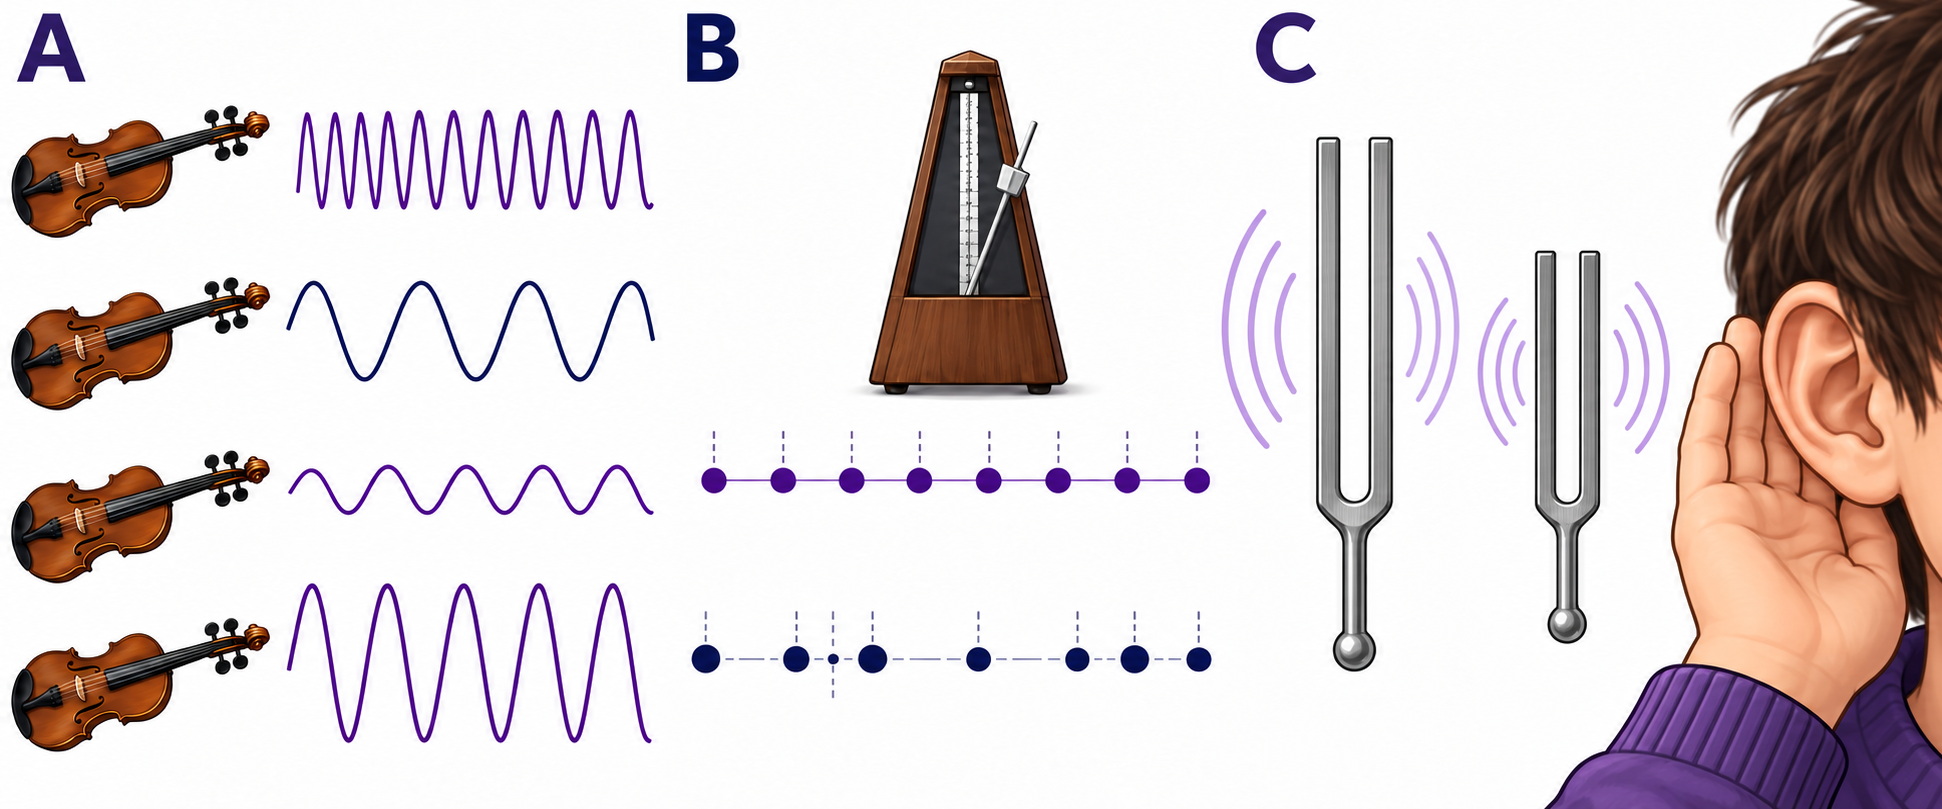
\includegraphics[width=\linewidth,height=0.26\textheight,keepaspectratio]{../assets/figure-f6141a0bb6d5.png}\par

{\small 本课重点看 A 区。A 比较振动疏密与振幅；B 稳定脉冲和节奏事件并不相同；C 两个音高之间可以比较方向与距离。波形仅作概念示意。}\par

{\footnotesize AI生成教学示意，非实物照片、原始史料或官方架构。生成方式：内置文生图；提示词见仓库 docs/image-prompts.json。}\end{center}

\Needspace{5\baselineskip}\section*{三个不同维度}

音高是我们对声音高低的感受，通常与振动频率密切相关。频率更高的纯音通常听起来更高；这不等于声音更大。[S1] 力度讨论演奏中的强弱及其变化，响度感受还受频率、音色与环境影响，因此图中振幅只能作简化提示。

音色帮助我们分辨“是谁在发声”：同一个音高由人声和小提琴发出，听感仍有差别。起音方式、泛音组成与声音随时间的变化都会影响音色。今天不要求记频谱术语，只要能说出尖锐、柔和、气声、拨弦等具体特征，同时承认这些描述有主观成分。

三个维度可以分别变化。轻声唱高音，音高升高而力度未必增加；同一音高逐渐唱强，力度变化却不必改变音高。实际演奏常把多项一起改变，因此观察时每次只追踪一个维度更容易。

\Needspace{5\baselineskip}\section*{读图与聆听方法}

图 A 上部用疏密对比提示音高，下部用振幅提示强弱；它不是真实乐器的声学测量。先哼一个舒适的音，再换到稍高的音，尽量保持强弱相近。接着固定音高，轻轻变强再变弱。若一开始做不到完全分离，很正常，目的在于意识到两种变化不同。

听熟悉歌曲前30秒，第一遍只跟人声高低，第二遍只听整体强弱，第三遍找一种伴奏声音。把结果写成三句话。即使不确定乐器名称，也可以写“短促、颗粒感的声音”，比猜一个专业名词更诚实。

\Needspace{5\baselineskip}\section*{三分钟练习与自查}

从三句描述中指出主要维度：“唱得越来越高”“同一个音逐渐变响”“钢琴换成人声唱同一段”。再描述你的短片段，每句话只写一个维度。

参考分别是音高、力度、音色。自查：有没有把高音等同于大声？有没有从音色直接断言某种情绪？若听不到明确人声，可以选一条持续的乐器线。今天不要求识别绝对音名，也没有标准审美答案。

\Needspace{5\baselineskip}\section*{复盘与明日连接}

欣赏音乐可以从可听见的变化开始：高低、强弱、声音质感。五线谱中的音符位置和时值只是记录部分信息的方式，不能把记谱当作声音本身。[S2] 明天把注意力从“什么声音”转向“声音何时发生”，学习节拍、节奏和速度。

\Needspace{6\baselineskip}\section*{扩展学习 / Further reading}\small 以下为选读，不计入每日必做时间。\begin{enumerate}[leftmargin=1.6em]

\item [S1] \href{https://openstax.org/books/physics/pages/14-1-speed-of-sound-frequency-and-wavelength}{Speed of Sound, Frequency, and Wavelength} — 选读声音频率与音高的关系，公式推导可跳过。\par OpenStax | 发布：未标注 | 核验：2026-10-08

\item [S2] \href{https://openmusictheory.github.io/basicNotation.html}{Basic notation} — 认识音符、谱表和变音记号；本课不要求记住全部符号。\par Open Music Theory | 发布：未标注 | 核验：2026-10-08

\item [S3] \href{https://openmusictheory.github.io/rhythmicValues.html}{Rhythmic values} — 观察长短时值和休止符如何表达时间。\par Open Music Theory | 发布：未标注 | 核验：2026-10-08

\item [S4] \href{https://openmusictheory.github.io/meter.html}{Meter and time signatures} — 选看拍子分组与聆听示例；部分嵌入播放器可能需要额外登录。\par Open Music Theory | 发布：未标注 | 核验：2026-10-08

\item [S5] \href{https://openmusictheory.github.io/intervals.html}{Intervals and dyads} — 重点看半音数与音程度数不是同一种计数方法。\par Open Music Theory | 发布：未标注 | 核验：2026-10-08

\end{enumerate}

\end{document}